\documentclass[tikz, border=1cm]{standalone}
\usepackage{pgfplots}
\pgfplotsset{compat=1.18}
\begin{document}
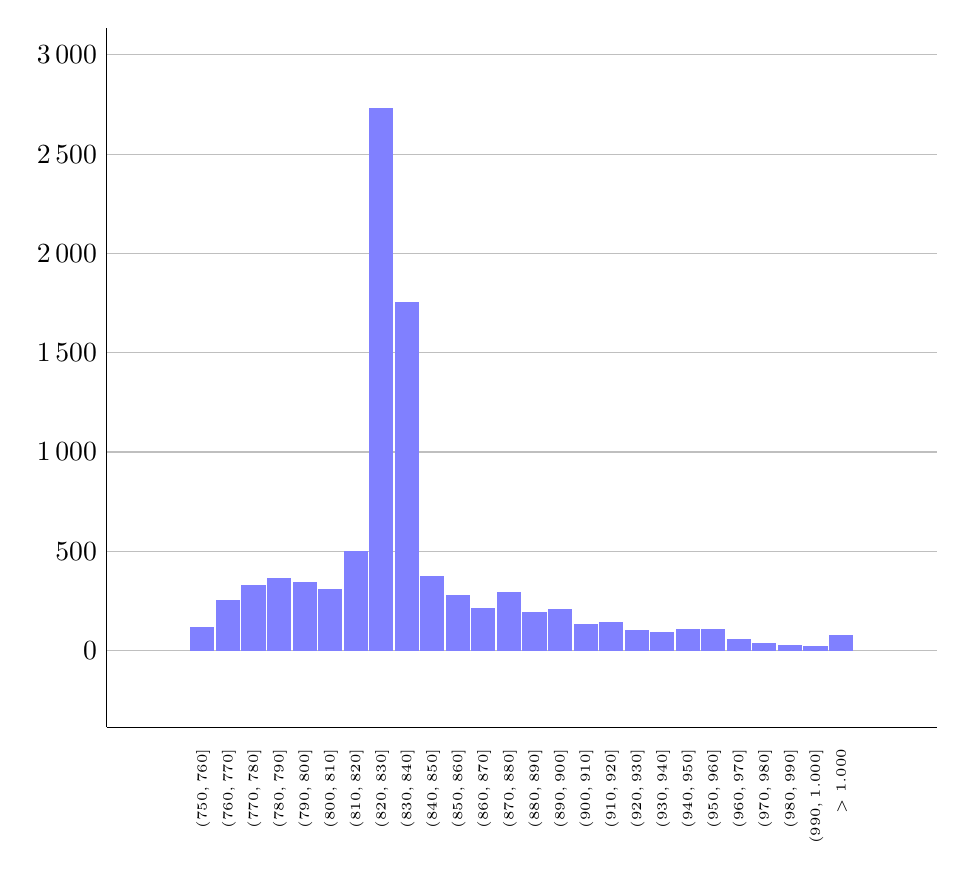
\begin{tikzpicture}
    \begin{axis}[
        ybar, bar width=9,
        ymajorgrids,
        axis lines*= left,
        width=\linewidth,
        xtick style= {draw=none}, ytick style= {draw=none},
        enlargelimits=0.15,
        xtick={750, 760, 770, 780, 790, 800, 810, 820, 830, 840, 850, 860, 870, 880, 890, 900, 910, 920, 930, 940, 950, 960, 970, 980, 990,1000},
        x tick label style = {rotate=90, yshift=1ex, font=\tiny},
        x tick label as interval=true,
        xticklabel={$(\pgfmathprintnumber{\tick}, \pgfmathprintnumber{\nexttick}]$},
        extra x ticks={1000,1010},
        extra x tick label={> \pgfmathprintnumber{\tick}},
        x tick label style = {/pgf/number format/set thousands separator={.}},
        y tick label style = {/pgf/number format/set thousands separator={\,}},
                 ]  
        \addplot[draw=blue!50, fill=blue!50] coordinates {(750,114) (760,252) (770,326) (780,363) (790,341) (800,306) (810,497) (820,2728) (830,1750) (840,372) (850,277) (860,210) (870,294) (880,191) (890,208) (900,129) (910,143) (920,98) (930,89) (940,103) (950,105) (960, 54) (970, 35) (980,24) (990,20) (1000,75)};   
    \end{axis}
\end{tikzpicture}
\end{document}
